\section{Receptor}
\label{sec:receptor}

\subsection{Diseño mecánico}
\label{sec:disenio_receptor}

Las piezas de la mano y de su soporte se diseñaron con Solid Edge, un programa de diseño asistido por computadora (CAD) desarrollado por Siemens.

\begin{figure}[H]
    \begin{center}
 		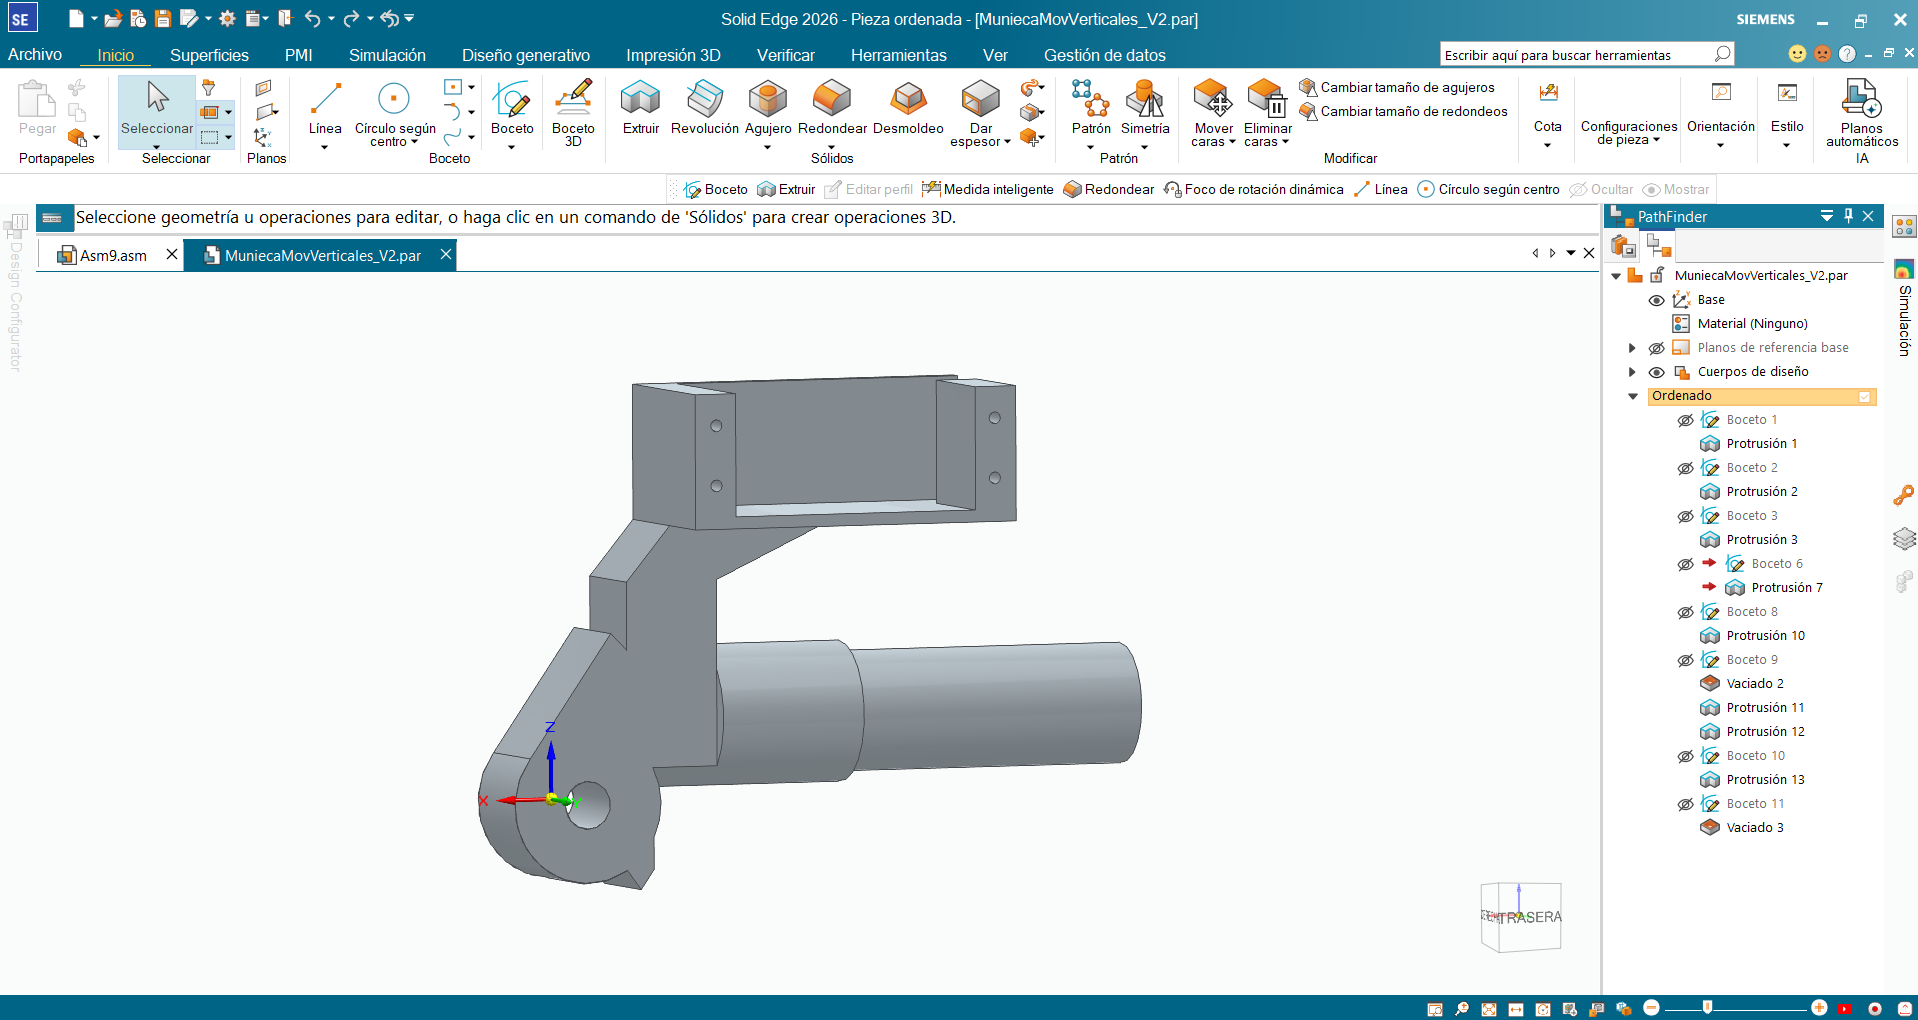
\includegraphics[scale=0.3]{SolidEdge.png}
 		\captionof{figure}{Entorno de Solid Edge.}
        \label{fig:SolidEdge}
    \end{center}
\end{figure}

En Solid Edge se dibujan bocetos en un plano y luego, mediante extrusiones, se los lleva de dos a tres dimensiones. Sobre una misma pieza se trazan bocetos en distintas caras y, con extrusiones, se realizan vaciados o protrusiones hasta obtener la forma deseada. De esta manera se desarrolló la estructura de la figura~\ref{fig:mano}.

\begin{figure}[H]
 \centering
  \subfigure[Vista lateral]{
    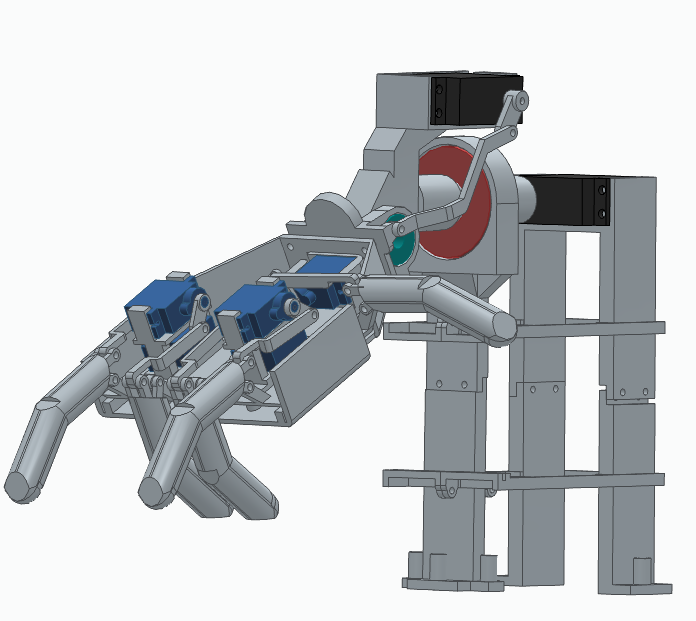
\includegraphics[width=0.42\textwidth]{Receptor/Receptor_1.png}}
  \subfigure[Vista posterior]{
    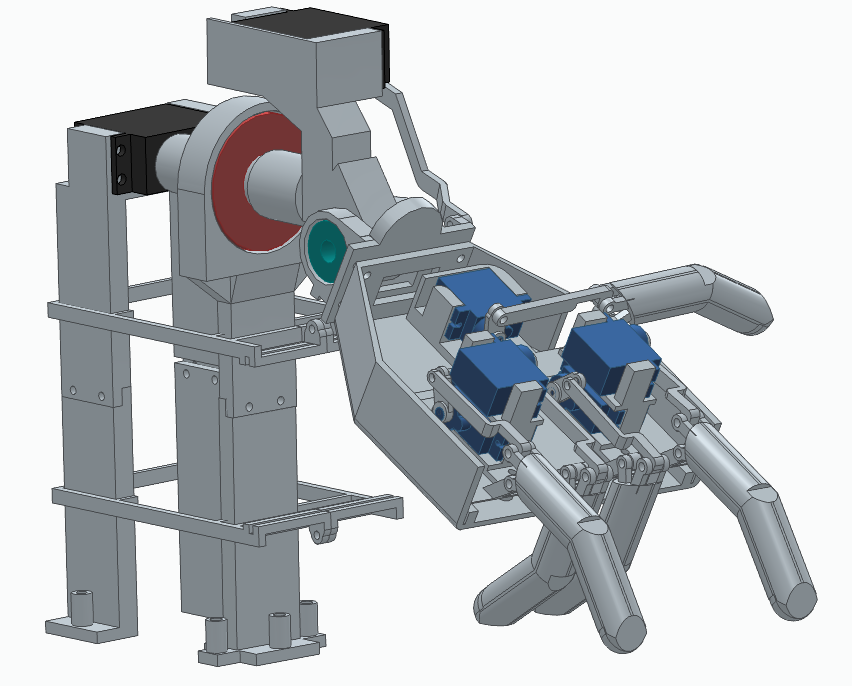
\includegraphics[width=0.48\textwidth]{Receptor/Receptor_2.png}}
 \caption{Diseño de la mano robótica y su soporte.}
 \label{fig:mano}
\end{figure}

La estructura se apoya sobre dos soportes de unos \SI{17}{\centi\meter} de altura. Para la rotación, un servo MG946R mueve un brazo de forma directa; para facilitar el giro se utiliza un rodamiento de \SI{20}{\milli\meter} de diámetro interior, y el brazo se une con la mano mediante un tornillo que pasa a través de ambos. El brazo contiene además el segundo servo MG946R, que mediante una biela produce el desplazamiento vertical de la mano.

Dentro de la palma, una base reúne los servos SG90 de los dedos. Los servos se ubican de a pares en forma vertical, uno en cada dirección, y cada uno se enlaza a su dedo mediante una biela; los dedos están atornillados a la base. El pulgar es la excepción: su servo se atornilla directamente a la base. También se diseñaron pequeños soportes que se enganchan a los soportes principales para sostener la base del microcontrolador. Todas las piezas se imprimieron en una impresora Hellbot Hidra.

\begin{figure}[H]
 \centering
  \subfigure[Muñeca]{
    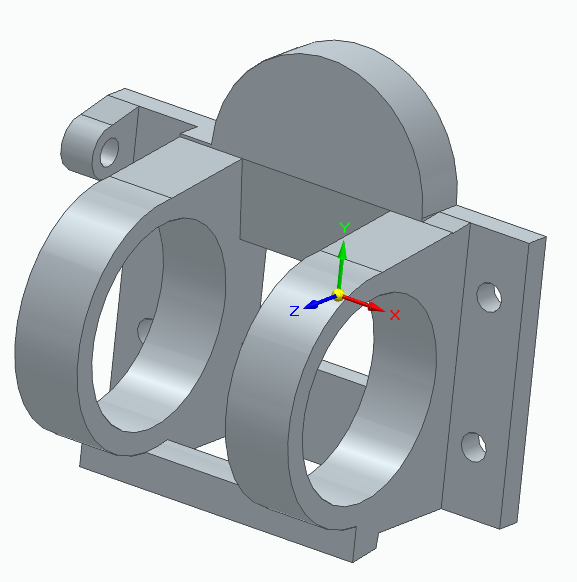
\includegraphics[width=0.22\textwidth]{Receptor/Muñeca.png}}
  \subfigure[Antebrazo]{
    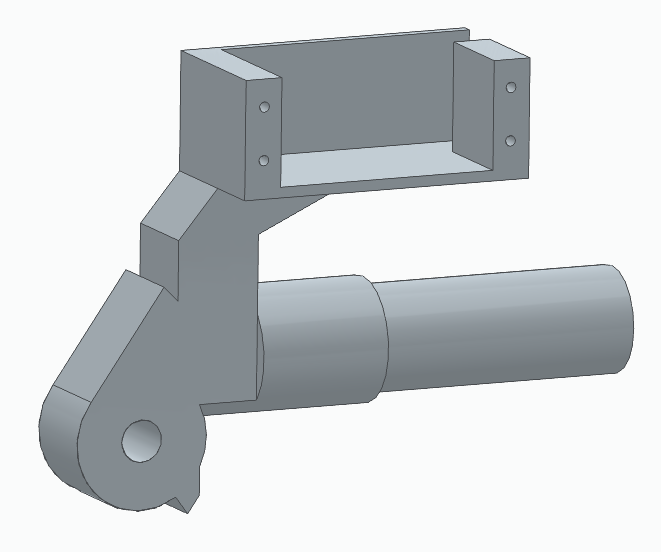
\includegraphics[width=0.22\textwidth]{Receptor/Antebrazo.png}}
  \subfigure[Palma]{
    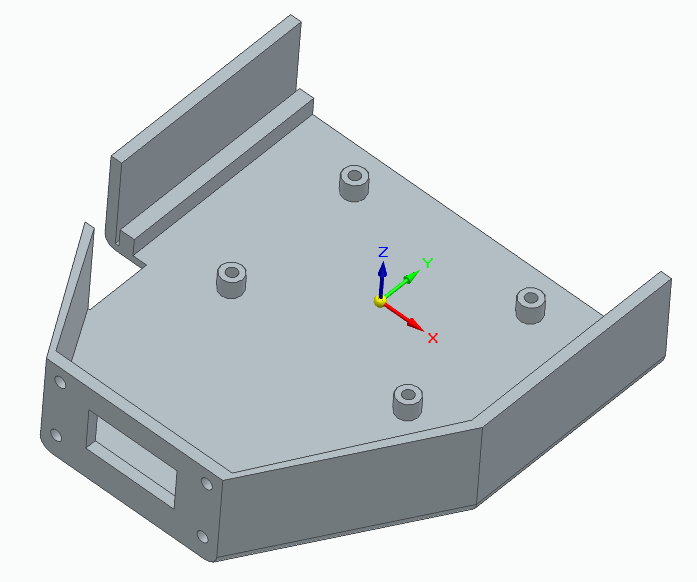
\includegraphics[width=0.22\textwidth]{Receptor/Palma.png}}
  \subfigure[Base de la mano]{
    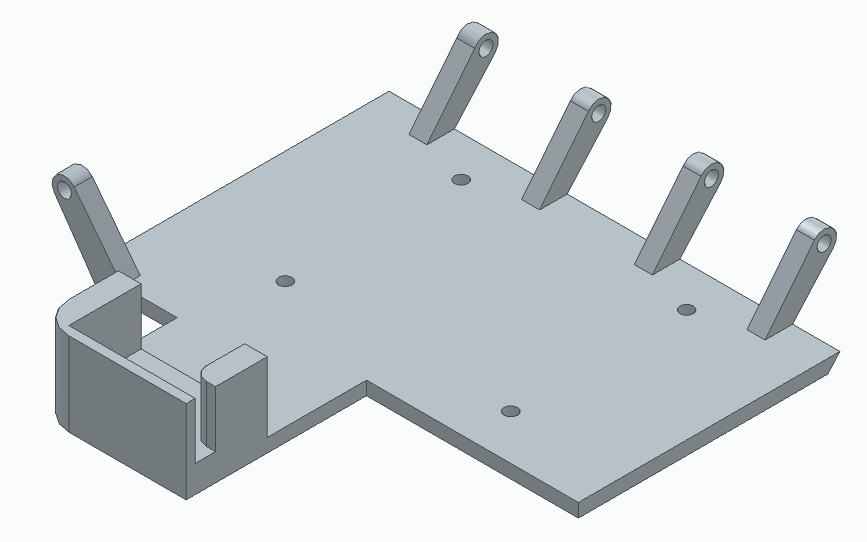
\includegraphics[width=0.22\textwidth]{Receptor/BaseMano.png}}
  \subfigure[Dedo]{
    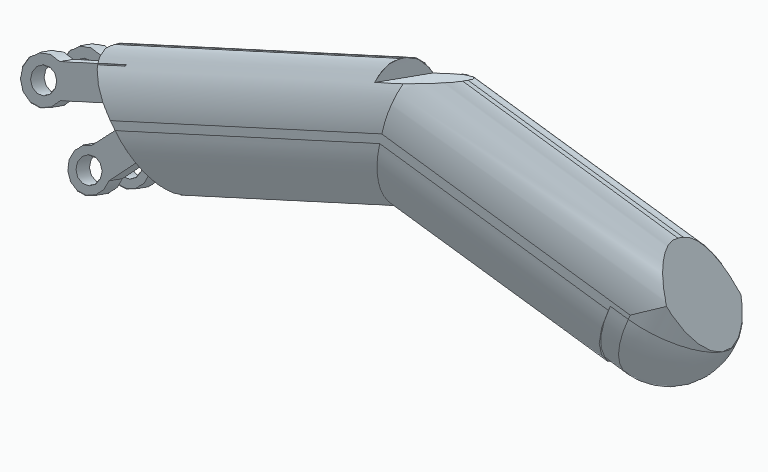
\includegraphics[width=0.22\textwidth]{Receptor/Dedo.png}}
  \subfigure[Base de servo]{
    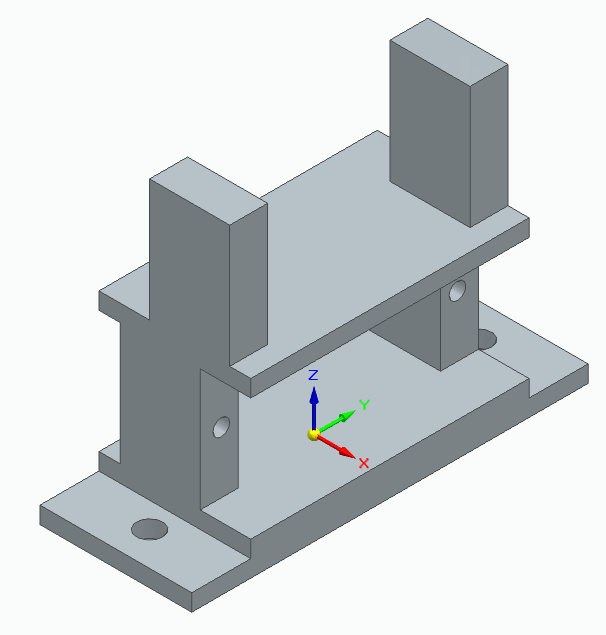
\includegraphics[width=0.22\textwidth]{Receptor/BaseServo.png}}
  \subfigure[Soporte]{
    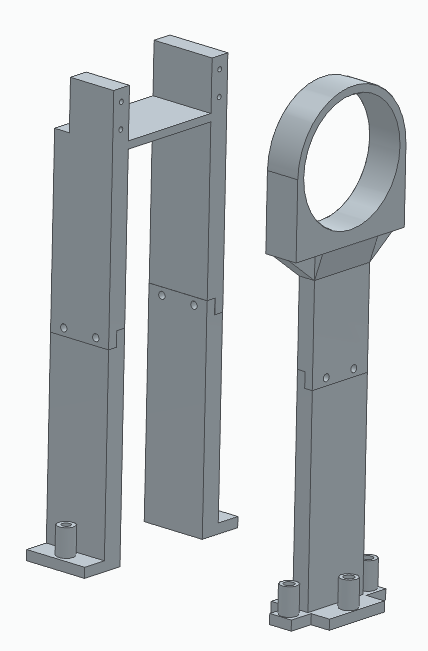
\includegraphics[width=0.22\textwidth]{Receptor/Soporte.png}}
 \caption{Piezas de la mano robótica.}
 \label{fig:piezas_mano}
\end{figure}

\pendiente{Revisar los nombres de las subfiguras y agregar una breve descripción de cada pieza si corresponde. Las imágenes \texttt{Diseño\_Receptor\_*.png} y \texttt{PrimerModeloMano\_*.png} quedaron sin usar: incluirlas si se quiere mostrar la evolución del diseño.}

\begin{figure}[H]
 \centering
  \subfigure[Base ESP32]{
    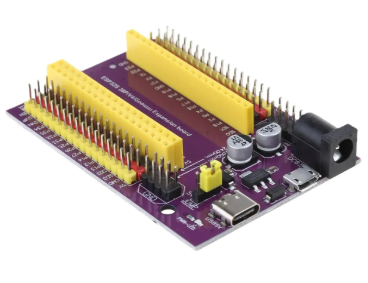
\includegraphics[width=0.3\textwidth]{ESP32_Base.png}}
  \subfigure[Impresora 3D Hellbot Hidra]{
    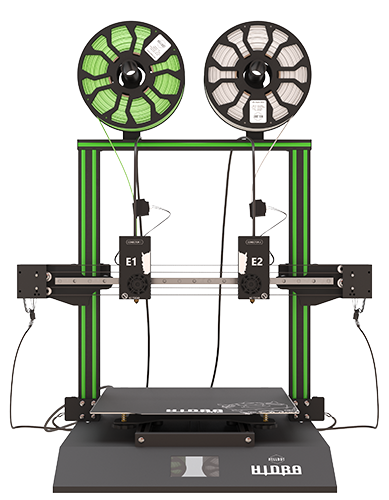
\includegraphics[width=0.2\textwidth]{Hidra_Hellbot.png}}
 \caption{Placa base del ESP32 e impresora utilizada.}
 \label{f:Extra}
\end{figure}

Como el software sólo limita los dedos al rango de \SIrange{25}{90}{\degree}, el diseño de las piezas debe permitir un recorrido libre algo mayor (por ejemplo, de \SIrange{20}{95}{\degree}), de manera que el servo nunca llegue a forzar la estructura de plástico y dañe sus engranajes.

\subsection{Conexionado y alimentación}
\label{sec:alimentacion}

El uso de la placa base del ESP32 (figura~\ref{f:Extra}) simplificó el conexionado, ya que ofrece tiras de pines con señal, alimentación y masa en la disposición que requieren los servos. La alimentación se dividió en dos:

\begin{itemize}
    \item \textbf{Servos:} una fuente externa de \SI{12}{\volt} y \SI{4}{\ampere} alimenta un regulador conmutado reductor (\textit{buck}) basado en el MP1584, cuya salida de \SI{5}{\volt} se conecta a los pines de alimentación de la placa base, de donde la toman los siete servos.
    \item \textbf{ESP32:} se alimenta por su conector micro-USB. Durante las pruebas lo alimenta la computadora, que también recibe la telemetría; en el diseño final se prevé un \textit{powerbank} o un paquete de baterías.
\end{itemize}

Las masas de ambas alimentaciones están unidas, ya que la señal PWM de cada servo se mide respecto del GND del ESP32. Para que las dos alimentaciones no queden conectadas entre sí, se removió el pin 5V de la placa del ESP32: de lo contrario, ese pin quedaría unido a los \SI{5}{\volt} de la placa base y el regulador podría inyectar corriente al puerto USB de la computadora.

\begin{figure}[H]
 \centering
  \subfigure[]{
    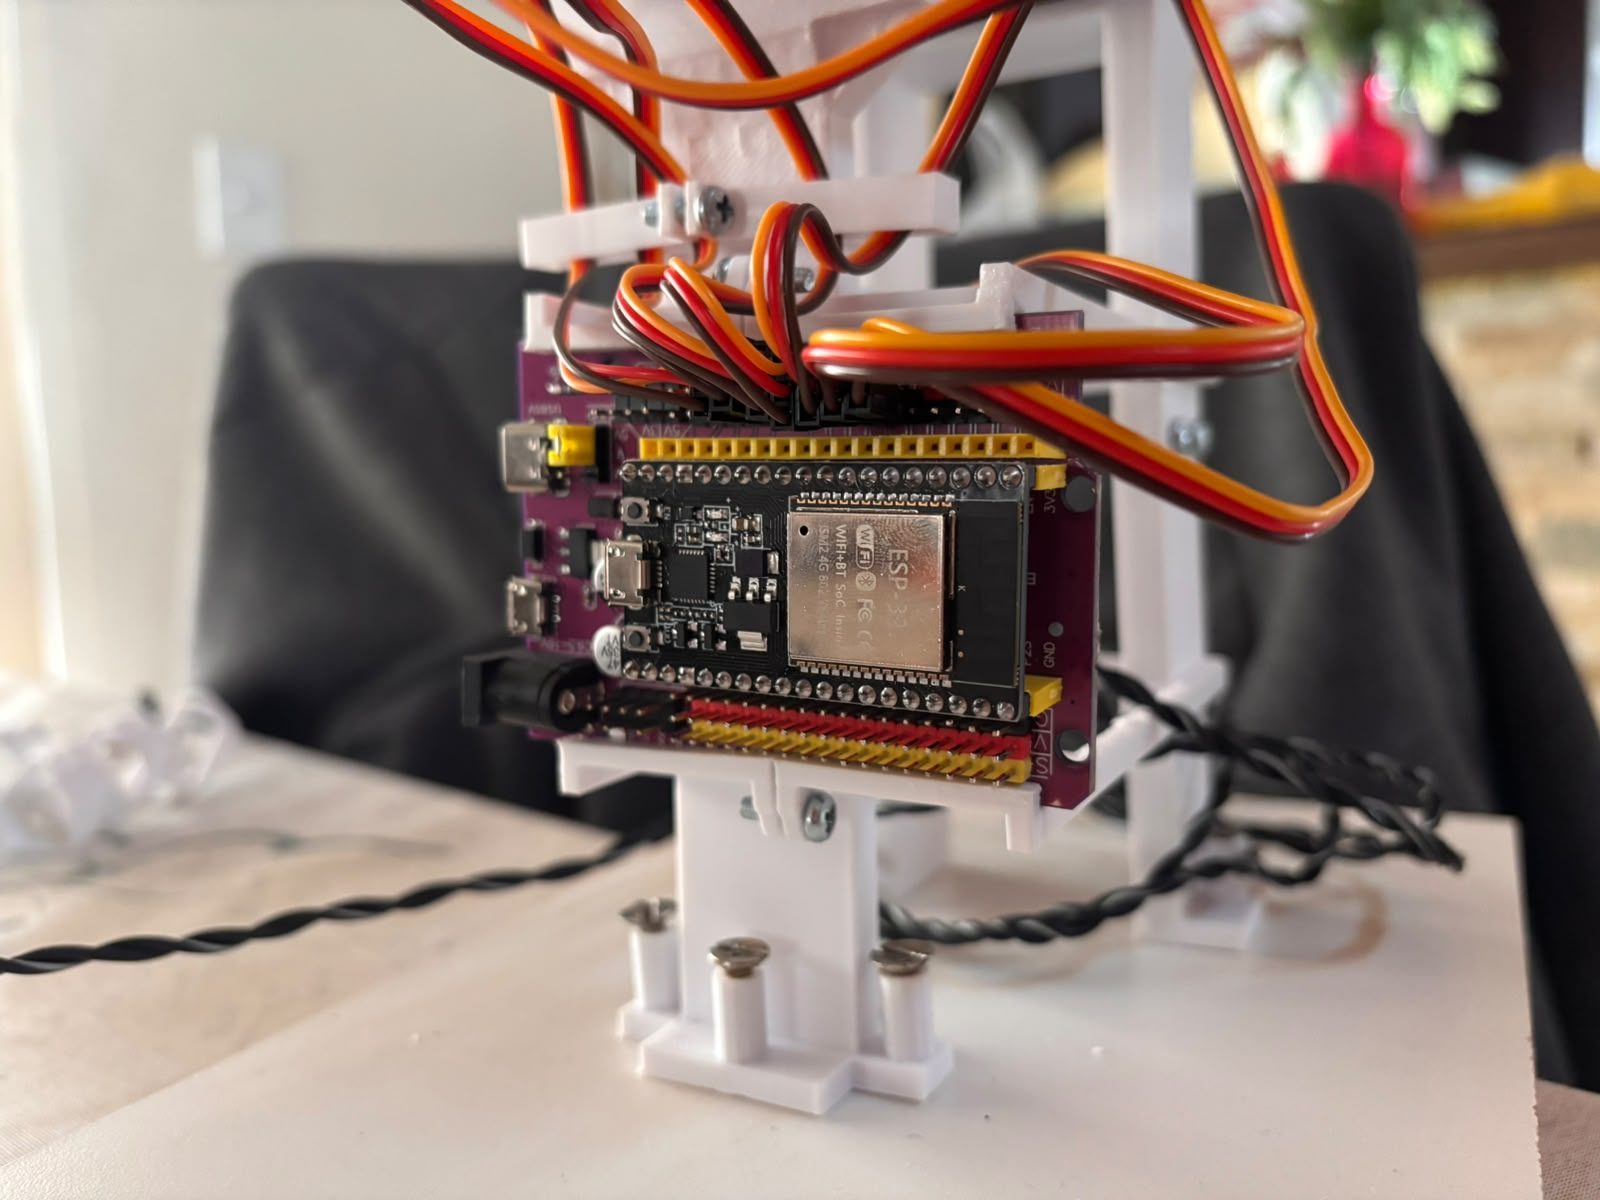
\includegraphics[width=0.45\textwidth]{Conexionado_Receptor_1.jpeg}}
  \subfigure[]{
    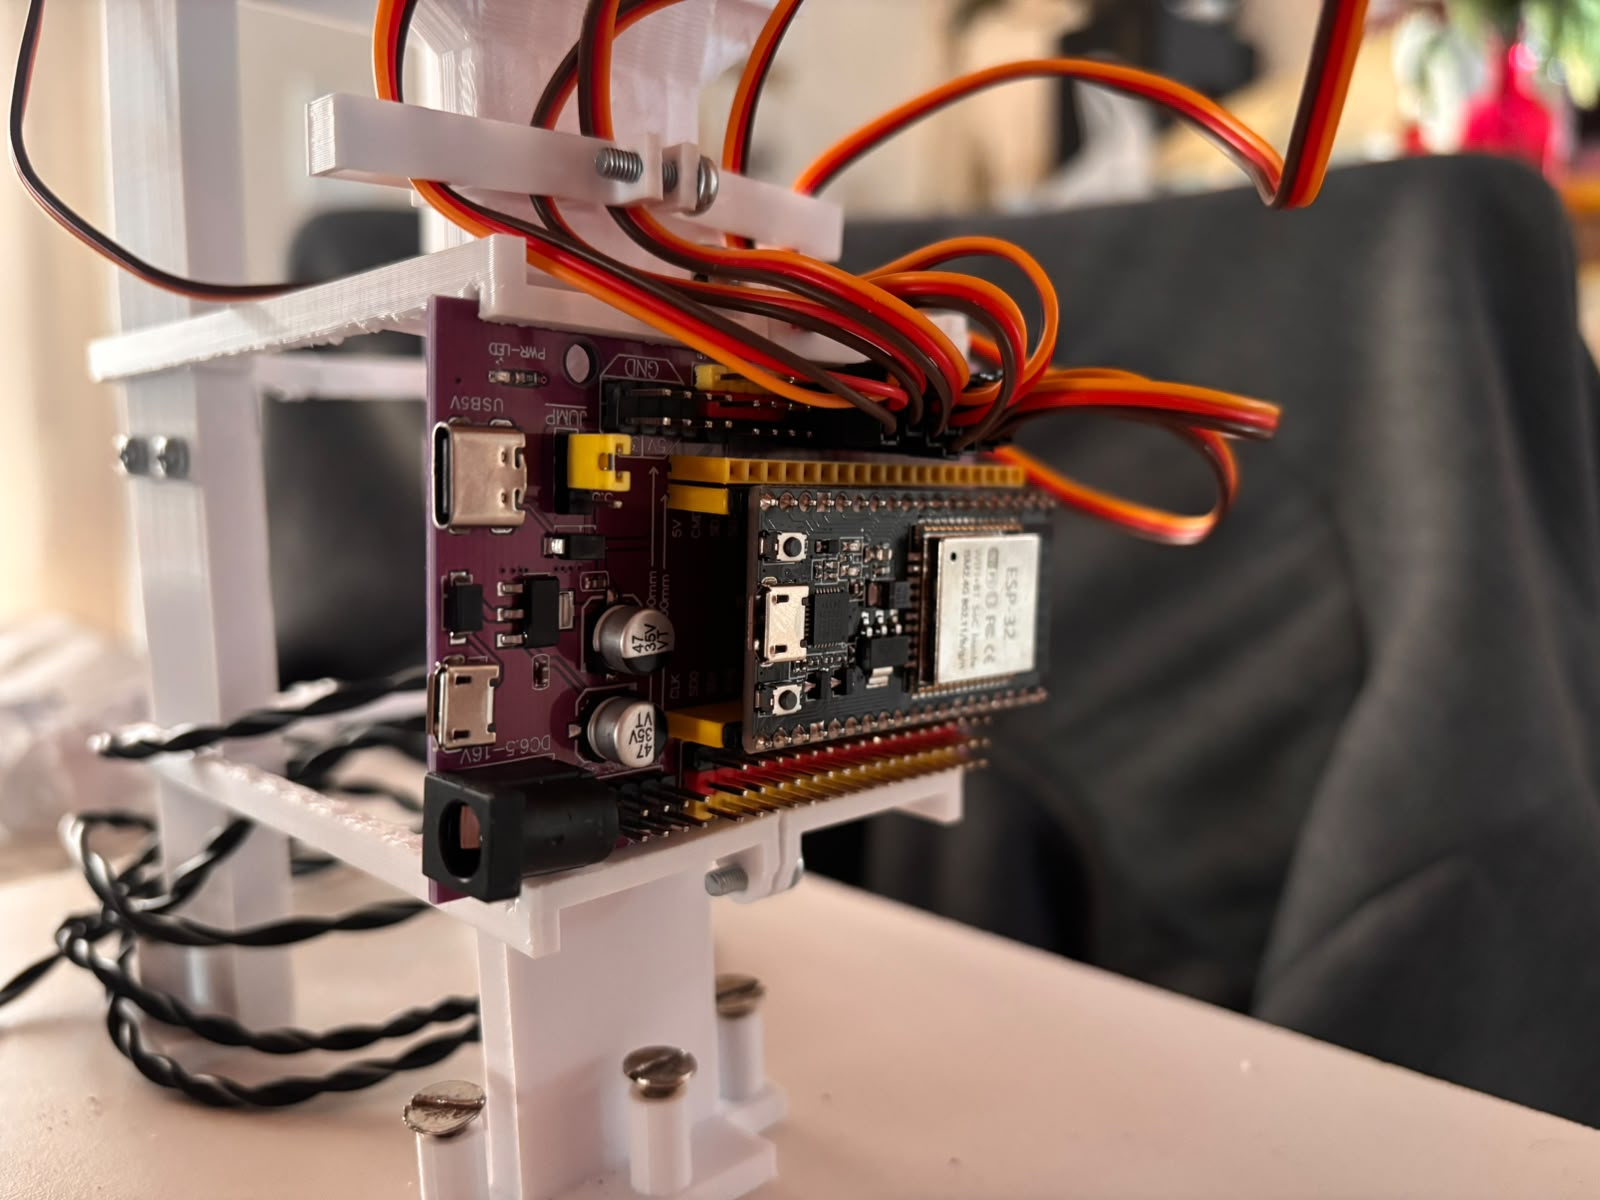
\includegraphics[width=0.45\textwidth]{Conexionado_Receptor_2.jpeg}}
 \caption{Conexionado del receptor.}
 \label{fig:conexionado_rx}
\end{figure}

La figura~\ref{fig:diagrama_rx} muestra el diagrama de conexionado del receptor, con las dos alimentaciones separadas.

\begin{figure}[H]
    \centering
    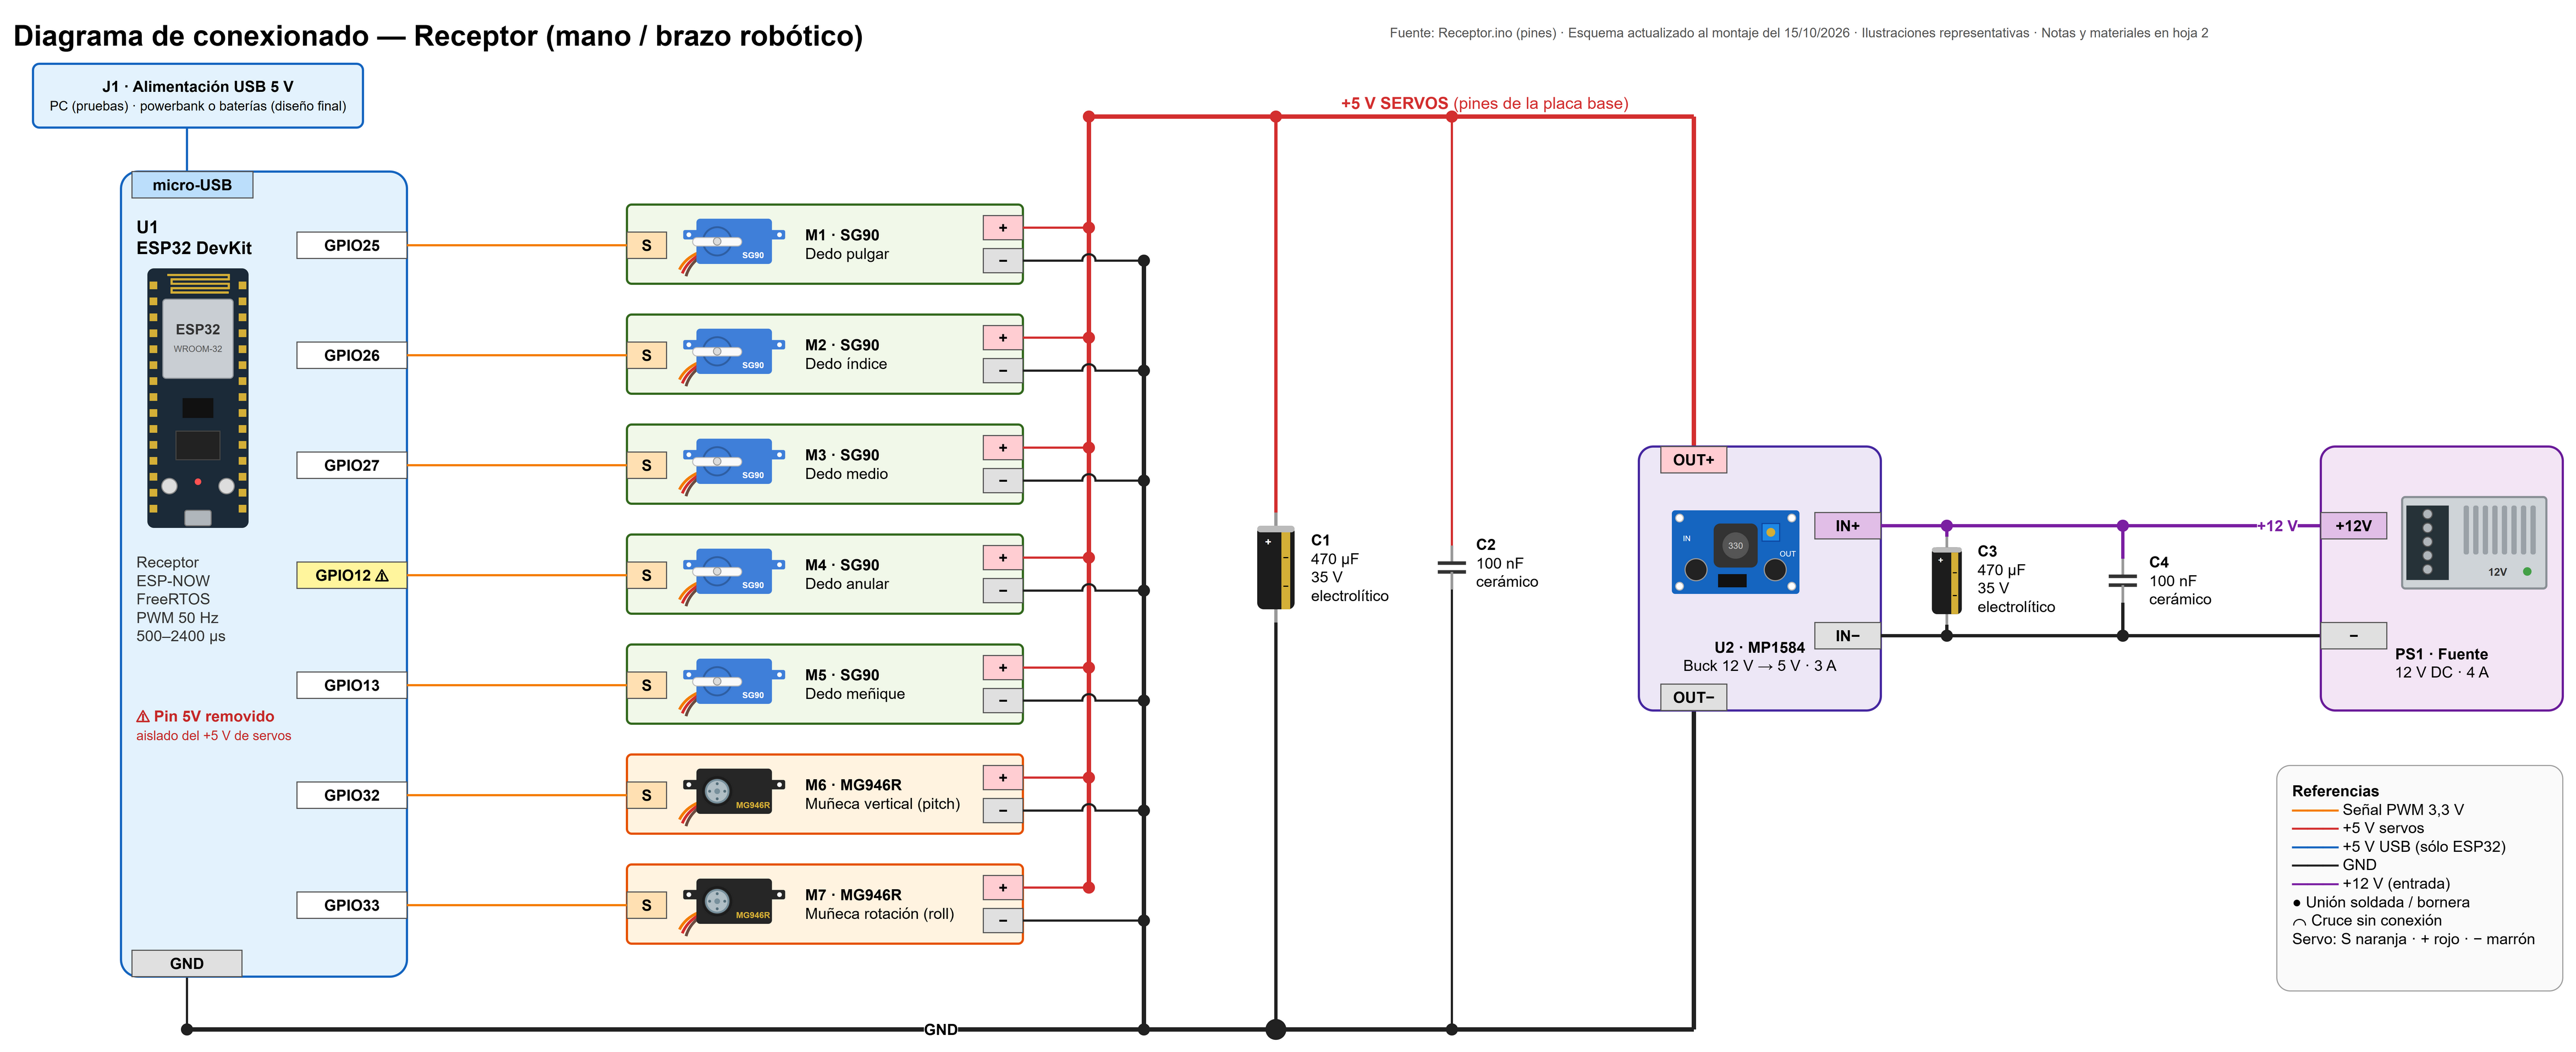
\includegraphics[width=\textwidth]{Conexionado_Receptor_Diagrama.png}
    \caption{Diagrama de conexionado del receptor.}
    \label{fig:diagrama_rx}
\end{figure}

La tabla~\ref{tab:pines_rx} indica el pin asignado a cada servo. Se eligieron los pines más cercanos a cada cable, ya que estos miden unos \SI{30}{\centi\meter} y no deben desconectarse cuando la mano se mueve.

\begin{table}[H]
\centering
\begin{tabular}{l c}
\toprule
\textbf{Servo} & \textbf{GPIO} \\
\midrule
Pulgar, índice, medio & 25, 26, 27 \\
Anular, meñique & 12, 13 \\
Muñeca vertical & 32 \\
Muñeca rotacional & 33 \\
\bottomrule
\end{tabular}
\caption{Asignación de pines del receptor.}
\label{tab:pines_rx}
\end{table}

El GPIO 12 es un pin de configuración de arranque (\textit{strapping}) del ESP32, que define la tensión de la memoria flash al iniciar \cite{esp32_datasheet}. Si se mantuviera en nivel alto durante el reinicio, la placa podría no arrancar. En las pruebas no causó inconvenientes, pero debe tenerse en cuenta ante una falla de arranque.

\begin{figure}[H]
    \begin{center}
 		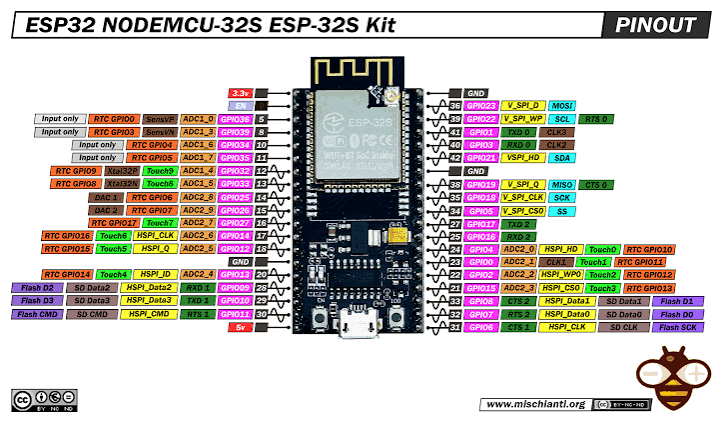
\includegraphics[scale=0.5]{ESP32_Pinout.png}
 		\captionof{figure}{Distribución de pines del ESP32.}
        \label{fig:pinout}
    \end{center}
\end{figure}

\subsubsection{Consumo}

La tabla~\ref{tab:consumos} resume los valores eléctricos de los componentes del receptor según sus fabricantes.

\begin{table}[H]
\centering
\begin{tabularx}{\textwidth}{l X X}
\toprule
\textbf{Componente} & \textbf{Valores} & \textbf{Fuente} \\
\midrule
SG90 (dedos) & \SI{4.8}{\volt}; \SI{1.8}{\kilo\gram\centi\meter} de torque de bloqueo. El fabricante no publica corrientes. Un distribuidor informa \SIrange{100}{250}{\milli\ampere} en movimiento y \SI{360}{\milli\ampere} bloqueado (medido por el distribuidor). & \cite{sg90_datasheet}, \cite{sg90_protosupplies} \\
MG946R (muñeca) & \SIrange{4.8}{6.6}{\volt}; \SI{10}{\milli\ampere} en reposo, \SI{170}{\milli\ampere} en operación sin carga y \SI{1.2}{\ampere} bloqueado; \SI{10.5}{\kilo\gram\centi\meter} a \SI{4.8}{\volt}. & \cite{mg946r_datasheet} \\
ESP32 & Alimentación del chip de \SIrange{2.3}{3.6}{\volt} (típica \SI{3.3}{\volt}); la fuente debe poder entregar al menos \SI{500}{\milli\ampere}. Consumo típico de la radio: \SI{240}{\milli\ampere} transmitiendo (802.11b, \SI{19.5}{dBm}) y \SIrange{95}{100}{\milli\ampere} recibiendo. & \cite{esp32_datasheet} (sec.~2.5.3, tablas 5-2 y 5-4) \\
MP1584 (regulador \textit{buck}) & Entrada de \SIrange{4.5}{28}{\volt}; \SI{3}{\ampere} de salida; frecuencia de conmutación programable de \SI{100}{\kilo\hertz} a \SI{1.5}{\mega\hertz}; límite de corriente del interruptor de \SI{4.0}{\ampere} mínimo (\SI{4.7}{\ampere} típico); apagado térmico a \SI{150}{\celsius}. & \cite{mp1584_datasheet} \\
\bottomrule
\end{tabularx}
\caption{Valores eléctricos de los componentes del receptor.}
\label{tab:consumos}
\end{table}

Para el SG90, la corriente de bloqueo varía entre fuentes no oficiales (de \SI{360}{\milli\ampere} a \SI{750}{\milli\ampere}), por lo que el valor medido en el propio montaje es más confiable que el de cualquier hoja de datos. Por otro lado, el valor mínimo de \SI{500}{\milli\ampere} del ESP32 cubre los picos de la radio (hasta \SI{379}{\milli\ampere} en transmisión continua según la hoja del módulo \cite{esp32_wroom_datasheet}).

Dado que los SG90 de los dedos no llegan al bloqueo, se los considera con consumo normal. En cambio, debe tenerse en cuenta la corriente de bloqueo de los MG946R, sobre todo la del servo de desplazamiento vertical, que es el que carga más peso. Considerando todo lo anterior, la fuente de los servos debe poder entregar al menos unos \SI{3}{\ampere}, que es la corriente nominal del MP1584. Con la corriente de bloqueo de los dos MG946R (\SI{2.4}{\ampere}) más el consumo de los cinco SG90 en movimiento, un pico simultáneo puede acercarse a ese valor o superarlo; por eso es importante limitar los picos.

Además del consumo medio, deben considerarse los picos de arranque: cuando varios servos arrancan a la vez, la corriente puede superar por algunos milisegundos la capacidad de la fuente. Si el ESP32 tomara su alimentación de esa misma línea de \SI{5}{\volt} y la tensión cayera lo suficiente, su regulador de \SI{3.3}{\volt} perdería regulación y el circuito de protección del microcontrolador provocaría un reinicio por baja tensión (\textit{brownout}); alimentarlo por USB separa su alimentación de la de los servos. Para limitar los picos se combinan dos medidas:

\begin{itemize}
    \item \textbf{En firmware}, el limitador de velocidad del receptor (sección~\ref{sec:slew}) impide que los servos reciban escalones grandes de posición, lo que reduce la aceleración pedida a los motores y, por lo tanto, los picos de corriente.
    \item \textbf{En hardware}, dos pares de capacitores iguales, cada uno formado por un electrolítico de \SI{470}{\micro\farad} / \SI{35}{\volt} en paralelo con un cerámico de \SI{100}{\nano\farad}:
    \begin{itemize}
        \item \textbf{A la salida del regulador}, sobre la línea de \SI{5}{\volt} de los servos y junto a los pines de la placa base. El electrolítico entrega la corriente de los picos de corta duración, que el regulador no alcanza a seguir, y el cerámico filtra el ruido de alta frecuencia que generan los motores y la conmutación del regulador.
        \item \textbf{A la entrada del regulador}, entre IN+ e IN$-$. Entrega los pulsos de corriente de la conmutación del regulador, de modo que la fuente de \SI{12}{\volt} y sus cables vean una corriente más pareja.
    \end{itemize}
\end{itemize}

El consumo medido sobre el montaje se presenta en la sección~\ref{sec:pruebas_alimentacion}. En resumen, a \SI{12}{\volt} el receptor consume en promedio unos \SIrange{75}{100}{\milli\ampere} en reposo y unos \SI{0.2}{\ampere} moviendo la muñeca en sus dos ejes, con picos de \SIrange{0.6}{0.7}{\ampere}. Estos valores están muy por debajo de los \SI{4}{\ampere} de la fuente y de los \SI{3}{\ampere} del regulador.

\subsection{Firmware del receptor}

\subsubsection{Arquitectura: callback, cola y tarea de control}

La figura~\ref{fig:arquitectura_rx} muestra el recorrido de un paquete dentro del receptor.

\begin{figure}[H]
\centering
\begin{tikzpicture}[node distance=0.6cm and 1.5cm, every node/.style={font=\small}]
  \node[bloque] (radio) {Radio\\ESP-NOW};
  \node[bloque, right=0.8cm of radio, fill=orange!10] (cb) {Callback\\\texttt{OnDataRecv}\\(tarea Wi-Fi, núcleo 0)\\Valida tamaño,\\firma y checksum};
  \node[bloque, right=of cb, fill=yellow!15] (cola) {Cola\\(1 elemento)};
  \node[bloque, right=of cola, fill=green!10] (ctrl) {Tarea de control\\(núcleo 1)\\Failsafe, trayectoria\\y escritura PWM};
  \node[bloque, below=of ctrl] (servos) {7 servos};
  \draw[flecha] (radio) -- (cb);
  \draw[flecha] (cb) -- node[below, font=\footnotesize]{sobrescribe} (cola);
  \draw[flecha] (cola) -- node[below, font=\footnotesize]{despierta} (ctrl);
  \draw[flecha] (ctrl) -- (servos);
\end{tikzpicture}
\caption{Recorrido de un paquete en el receptor.}
\label{fig:arquitectura_rx}
\end{figure}

\paragraph{Recepción.} El callback de recepción de ESP-NOW se ejecuta dentro de la tarea de Wi-Fi \cite{espnow_idf}, por lo que debe ser breve: descarta los paquetes cuyo tamaño no es de 19 bytes o cuya firma o suma de verificación no son válidas, y copia el paquete válido en una cola de FreeRTOS.

\paragraph{Cola de un elemento.} Si el callback escribiera directamente las variables que usa la tarea de control, ésta podría leer un paquete a medio escribir (condición de carrera). La cola copia el paquete completo de forma atómica. Su longitud es uno y se escribe con \texttt{xQueueOverwrite}, de modo que funciona como un buzón que guarda sólo el último paquete \cite{freertos}: si llegan dos antes de que la tarea los lea, el más viejo se descarta en lugar de acumularse, lo que generaría un retardo creciente.

\paragraph{Tarea de control.} La tarea queda bloqueada esperando la cola durante, como máximo, \SI{20}{\milli\second}. Si llega un paquete, despierta en ese mismo instante y lo procesa; si no llega ninguno, el tiempo de espera vence y la tarea itera igual, de modo que la supervisión del enlace y el movimiento hacia la posición de reposo siguen funcionando a \SI{50}{\hertz}.

\begin{lstlisting}[caption={Espera de paquetes en la tarea de control.}, label={cod:cola}]
if (xQueueReceive(colaMensajesBrazo, &paqueteEntrante,
                  pdMS_TO_TICKS(PERIODO_CONTROL_MS)) == pdTRUE) {
    marcaTiempoUltimoPaquete = millis();
    // ... pasar a operación normal si hacía falta y actualizar objetivos
    posObjetivoMuniecaVert = constrain((float)paqueteEntrante.muniecaVertical,
                                       LIM_MUNIECA_VERT_MIN, LIM_MUNIECA_VERT_MAX);
}
\end{lstlisting}

Al recibir un paquete, las posiciones objetivo se saturan a los límites mecánicos de la mano (\SIrange{25}{90}{\degree} para los dedos y la muñeca vertical, \SIrange{0}{180}{\degree} para la rotación), como protección adicional ante un valor fuera de rango.

\subsubsection{Máquina de estados y modo de seguridad}
\label{sec:fsm}

La tarea de control supervisa el enlace con la máquina de estados de la figura~\ref{fig:fsm}.

\begin{figure}[H]
\centering
\begin{tikzpicture}[node distance=1.6cm and 2.2cm, every node/.style={font=\small},
  estado/.style={draw, rounded corners=8pt, align=center, minimum width=3cm, minimum height=1.1cm, fill=blue!5}]
  \node[estado] (sync) {\texttt{ESPERANDO\_SYNC}\\Servos en reposo};
  \node[estado, right=of sync, fill=green!10] (normal) {\texttt{OPERACION\_NORMAL}\\Sigue al guante};
  \node[estado, below=of normal, fill=red!10] (fs) {\texttt{FAILSAFE\_SIN\_SENAL}\\Objetivos en reposo};
  \node[estado, right=of fs, fill=gray!15, dashed] (desac) {Servos desacoplados\\(sin PWM)};
  \draw[flecha] ($(sync.north)+(0,0.7)$) -- node[right, font=\footnotesize]{Inicio} (sync);
  \draw[flecha] (sync) -- node[above, font=\footnotesize]{Paquete válido} (normal);
  \draw[flecha] ($(normal.south)+(0.5,0)$) -- node[right, font=\footnotesize, align=left]{$>\SI{250}{\milli\second}$\\sin paquetes} ($(fs.north)+(0.5,0)$);
  \draw[flecha] ($(fs.north)+(-0.5,0)$) -- node[left, font=\footnotesize]{Paquete válido} ($(normal.south)+(-0.5,0)$);
  \draw[flecha] (fs) -- node[above, font=\footnotesize, align=center]{En reposo y\\$>\SI{2}{\second}$} (desac);
  \draw[flecha] (desac.north) |- node[pos=0.25, right, font=\footnotesize, align=left]{Paquete válido\\(reacopla)} (normal.east);
\end{tikzpicture}
\caption{Máquina de estados del receptor. El estado ``desacoplado'' no es un estado del código: es el modo de seguridad con los servos apagados.}
\label{fig:fsm}
\end{figure}

\begin{itemize}
    \item Al encender, los servos se energizan en la posición de reposo (dedos en \SI{25}{\degree}, muñeca vertical en \SI{57}{\degree} y rotación en \SI{90}{\degree}) y se espera el primer paquete válido.
    \item Si en operación normal pasan más de \SI{250}{\milli\second} sin paquetes válidos (unos 12 paquetes perdidos seguidos), se considera perdido el enlace: por ejemplo, porque el guante se apagó o salió de alcance. Las posiciones objetivo pasan a la de reposo y la mano se mueve hacia ella de forma suave. Este tiempo tolera interferencias breves y reacciona rápido ante un corte real.
    \item Si el modo de seguridad se mantiene, todos los servos llegaron a la posición de reposo y pasaron más de \SI{2}{\second} desde que se entró en él, se interrumpe la señal PWM (\texttt{detach}). Sin señal, los servos dejan de sostener la posición, de consumir corriente y de calentarse.
    \item En cualquier caso, al llegar un paquete válido se vuelve a operación normal y, si hacía falta, se vuelven a acoplar los servos, que arrancan desde la última posición escrita para no dar un salto.
\end{itemize}

\subsubsection{Generador de trayectoria: limitador de velocidad y banda muerta}
\label{sec:slew}

En cada iteración, para cada servo $i$, se calcula el error entre la posición objetivo y la actual y se avanza a lo sumo $\Delta\theta_{\max}$ grados:
\begin{equation}
e_i[k] = \theta^{obj}_i - \theta_i[k-1], \qquad
\theta_i[k] =
\begin{cases}
\theta_i[k-1] + \operatorname{sat}_{[-\Delta\theta_{\max},\,\Delta\theta_{\max}]}\left(e_i[k]\right) & \text{si } |e_i[k]| > \delta \\
\theta_i[k-1] & \text{si } |e_i[k]| \leq \delta
\end{cases}
\end{equation}

\paragraph{Limitador de velocidad (\textit{slew-rate limiter}).} Ante un salto grande del objetivo, por ejemplo al reconectarse o al entrar en el modo de seguridad, el movimiento resultante es una rampa y no un escalón. Esto limita los picos de corriente y el esfuerzo sobre los engranajes y las piezas impresas. Los límites elegidos (tabla~\ref{tab:param_rx}) son cercanos a la velocidad propia de los servos, de modo que en uso normal casi no agregan retardo.

\paragraph{Banda muerta (\textit{deadband}).} Si el error es menor o igual a $\delta$ no se escribe una nueva posición. Sin esta banda, el ruido residual del guante haría que el servo corrija décimas de grado constantemente y zumbe (\textit{hunting}), calentándose. Como contrapartida, la posición final puede diferir del objetivo hasta en $\delta$.

\begin{table}[H]
\centering
\begin{tabular}{l c c c}
\toprule
\textbf{Servo} & $\boldsymbol{\Delta\theta_{\max}}$ \textbf{por ciclo} & \textbf{Velocidad máxima} & \textbf{Banda muerta} $\boldsymbol{\delta}$ \\
\midrule
Dedos (SG90)              & \SI{8}{\degree} & \SI{400}{\degree\per\second} & \SI{1.0}{\degree} \\
Muñeca vertical (MG946R)  & \SI{4}{\degree} & \SI{200}{\degree\per\second} & \SI{1.2}{\degree} \\
Muñeca rotacional (MG946R)& \SI{5}{\degree} & \SI{250}{\degree\per\second} & \SI{1.2}{\degree} \\
\bottomrule
\end{tabular}
\caption{Parámetros del generador de trayectoria (ciclo de \SI{20}{\milli\second}).}
\label{tab:param_rx}
\end{table}

\subsubsection{Inversión del sentido de los dedos}

Todo el sistema trabaja con la convención lógica de \SI{25}{\degree} = dedo abierto y \SI{90}{\degree} = dedo cerrado. Según cómo esté montado cada servo en la palma, puede ocurrir que cierre el dedo al \emph{disminuir} su ángulo. Para no modificar la mecánica, el arreglo \texttt{INVERTIR\_DEDO} indica, para cada dedo, si el ángulo debe espejarse dentro del rango justo antes de escribirlo en el servo:
\begin{equation}
\theta_{servo} =
\begin{cases}
25 + 90 - \theta & \text{si el dedo está invertido} \\
\theta & \text{en otro caso.}
\end{cases}
\end{equation}
Como la inversión se aplica sólo en la escritura, la posición de reposo, los límites, el modo de seguridad y la telemetría siguen expresados en la convención lógica.

\subsubsection{Generación de PWM}

Los servos se controlan con la librería \texttt{ESP32Servo}, que genera la señal con el periférico LEDC del ESP32. Al inicio se reservan cuatro temporizadores de hardware para este fin. Cada servo se configura a \SI{50}{\hertz} con pulsos de \SI{500}{\micro\second} para \SI{0}{\degree} y \SI{2400}{\micro\second} para \SI{180}{\degree}, es decir, unos \SI{10.6}{\micro\second} por grado.
